\subsubsection{Externe Schnittstellen}
Der FreeDesign-Editor kommuniziert über folgende vier Schnittstellen:
\begin{itemize}
	\item Über eine grafische Oberfläche wird der Editor vom Nutzer bedient und die Anwendung reagiert sowohl auf Mauseingaben als auch auf Tastatureingaben. 
	\item Zur Kommunikation mit Unitedprint-Backend wird eine REST-API genutzt. 
	\item Der Editor wird mit einer Reihen von URL-Parametern aufgerufen, die steuern, welche Produkt-Konfiguration von der Anwendung geladen wird. Über die URL-Parameter kann auch das Laden von Designvorlagen oder Kundendesign gesteuert, sowie weiter Funktionalitäten des Editors aktiviert werden. 
	Innerhalb des Editor besteht auch die Möglichkeit das Produkt zu ändern, worauf hin die URL sich aktualisiert.
	\item Ein Browser-Cookie wird vorwiegend zur Nutzer-Authentifizierung genutzt. 
\end{itemize}

Browser bieten die Möglichkeiten Daten in einem Local-Storage-Object oder einem Session-Storage-Object Daten zu speichern. \autocite[vgl.][]{Mozilla:Storage}
Die werden jedoch aktuell von der Anwendung nicht genutzt. 

% TODO: Es fehlt das Clipboard

\begin{figure}[H]
    \centering
    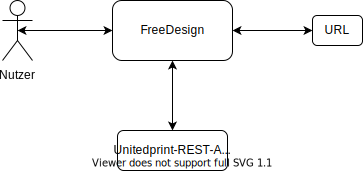
\includegraphics{diagrams/Ist-Architektur/Freedesign_Interaktion.pdf}
     \caption{Externe Schnittstellen}
     \label{fig:Externe_Schnittstellen}
  \end{figure}
  